\begingroup
\newcommand{\GerlingSeconds}[2]{#1\makebox[.42em][c]{,\makebox[0pt][r]{\textsuperscript{s}}}#2}
\begin{center}
\textsc{Gauss} an \textsc{Gerling}.\quad Göttingen, 11.~August 1823.
\end{center}

\par\noindent\hspace*{\parindent}\mbox{.\ .\ .\ .\ .\ .\quad Ihr} Ausdruck, \textls[120]{wenn} ich vom Brocken aus auf Heliotroplicht pointiren wolle und nicht das Häuschen vorzöge etc., scheint auf einiges Missverständniss der Motive, um derenwillen ich zum zweiten Male auf den Brocken gehen könnte, hinzudeuten.
Die scharfe Bestimmung der Richtung zum Inselsberg ist in der That ein Hauptzweck, und von Pointiren auf das Haus kann bei dieser Entfernung und der geringen Höhe und Irregularität desselben gar keine Rede sein.
Heliotroplicht vom Inselsberg zum Brocken ist also natürlich die Conditio sine qua non meines Hingehens.
\par\noindent\hspace*{\parindent}Dieser Eine Grund allein würde mich jedoch noch nicht wegen des abermaligen Besuchs rechtfertigen.
Meine Winkelmessungen 1821 nach meinen
\par\clearpage
\noindent\null\hfill{\small\textbf{ZUR HANNOVERSCHEN TRIANGULATION.}}\hfill\makebox[0pt][r]{\fontsize{13}{16}\selectfont 383}\par\medskip
\noindent eigenen Hauptpunkten waren bei dem ambulirenden Heliotrop und ungünstigen Wetter zu dürftig und des Ganzen nicht völlig würdig ausgefallen; daher ich diese durch gleichzeitige Besetzung mit Heliotropen wiederholen, wie nachher auch noch einmal zum Hohehagen und Hils zurückzukehren wünschte.
\par\noindent\hspace*{\parindent}So wie ich nun mit grösstem Vergnügen vom Brocken und Hohehagen zum Inselsberg Licht für Licht zu schicken erbötig bin, so bin ich doch nicht im Stande, Ihnen einen meiner Heliotropen hiebei abzulassen; denn wenn ich Hohehagen, Hils und vielleicht Lichtenberg durch einen ambulirenden besetzen müsste, so käme ich nicht weiter als 1821.
\par\noindent\hspace*{\parindent}Es scheinen mir nun mehrere Wege, wie hier durchzukommen ist, denkbar:
\par\noindent\hspace*{\parindent}1) Kommen wir gleichzeitig resp. zum Inselsberg und Brocken und schicken uns gegenseitig Licht, so wie mein Gehülfe Ordre haben soll, Ihnen von Zeit zu Zeit Licht vom Hohehagen, und der Ihrige mir vom Meisner zu schicken, so kann ich unter Begünstigung des Wetters, wie es Anfang September häufig ist, in wenigen Tagen, vielleicht in dreien, auf dem Brocken fertig werden, den Gehülfen mit dem Heliotrop dort lassen (der fortwährend Ihnen zum Inselsberg Licht schickt, so wie der auf dem Hohehagen), zum Hohehagen eilen, Ihnen Zeichen meiner Ankunft geben und wieder in ein paar Tagen (unter Gunst des Wetters) dort das zum Inselsberg gehörige absolviren, worauf Sie dann über Ihren Inselsberg-Heliotrop nach Gefallen disponiren können.
Vom Hohehagen erhalten Sie dann \textls[120]{beständig} Licht, so lange ich da bin, und wenn Sie es noch bedürfen, ab und an, so bald ich auf dem Hils bin.
\par\noindent\hspace*{\parindent}In Beziehung auf diesen Plan wird also alles darauf ankommen, ob Sie die Verbindung mit dem Brocken und den hannoverschen Dreiecken für wichtig genug halten, die Besetzung des Knills und der Milseburg mit Heliotropen so lange aufzuschieben, bis jener effectuirt ist.
\par\noindent\hspace*{\parindent}2) Obgleich der oben angezeigte Weg mir der liebste wäre, insofern dadurch die Verbindung der Messungen am vollkommensten effectuirt wird, so könnten Sie doch den Inselsberg-Heliotrop \textls[120]{allenfalls} schon früher abgeben, nemlich so bald ich den Brocken verlasse, was durch Signale kundgemacht werden kann.
In Beziehung auf die Richtung Hohehagen-Inselsberg müsste ich mich dann mit dem begnügen, was ich 1821 durch \textsc{Enckes} Helio-
\par\clearpage
\noindent\makebox[0pt][l]{\fontsize{13}{16}\selectfont 384}\hfill{\small\textbf{BRIEFWECHSEL MIT GERLING.}}\hfill\null\par\medskip
\noindent trop erhalten habe.
Es versteht sich, dass Sie die Lage des neuen Steins und Heliotropplatzes gegen das \textls[120]{Haus} auf das schärfste bestimmen müssten.
Ich wiederhole jedoch, dass es besser sein würde, wenn ich den Winkel vom Inselsberg zum Brocken auf dem Hohehagen unmittelbar erhalten könnte.
\par\noindent\hspace*{\parindent}3) Am allerbesten wäre es wohl, wenn Sie sogleich sich noch einen dritten Heliotrop anschafften.
Der kleine Aufwand würde gewiss reichlich durch den Genauigkeits- und Zeitgewinn überwogen, den Sie künftig davon haben würden.
Dies ginge jetzt um so leichter an, da \textsc{Rumpf} eben einen neuen Heliotrop fertig stehen hat.
Er hat nemlich einen für \textsc{Schumacher} verfertigt (und bereits abgesandt) und bei der Gelegenheit, weil, wie er sagt, es sich leichter arbeiten lässt, sogleich zwei auf einmal gearbeitet.
Der zweite ist also in diesem Augenblick noch disponibel, obwohl nicht zu zweifeln ist, dass er auch sonst leicht Gelegenheit finden wird, ihn abzusetzen.
(Bei mir sind bereits mehrere Anfragen aus dem Auslande eingegangen.)
Ich habe Hrn.~\textsc{Rumpf} ersucht, diesen Heliotrop theils ganz versendungsfertig zu machen, theils ihn nicht eher an sonst jemand wegzugeben, bis Ihre Erklärung darauf erfolgt sein würde.
Wenn Sie darauf reflectiren, so ist vielleicht das sicherste und kürzeste, ihn nach dem Meisner schicken oder abholen zu lassen.
\par\noindent\hspace*{\parindent}4) Ich könnte auch etwas früher nach dem Brocken, als Sie nach dem Inselsberge, abgehen; Sie müssten auf der Milseburg also suchen, die Richtung zum Inselsberg vor allen andern zu erhalten, damit von dem zu verabredenden Tage an, wo ich auf dem Brocken eintreffe, Ihr Gehülfe vom Inselsberg mir fortwährend Licht zum Brocken schickt.
So würden Sie Ihren Heliotrop auf dem Inselsberg eine kürzere Zeit nach Ihrer eigenen Ankunft zu behalten nöthig haben.
\par\noindent\hspace*{\parindent}Sollte aber alles dieses mit Ihren Plänen nicht vereinbar sein, so würde ich von der ganzen Expedition, für dies Jahr wenigstens, abstrahiren müssen (in welchem Fall ich aber um möglichst baldige Benachrichtigung bitte, damit ich und meine Gehülfen uns danach einrichten können); auch weiss ich nicht, ob ich im künftigen Jahre im Stande sein würde, mich in demselben Maasse einrichten zu können wie diesmal.
Diesmal nemlich erbiete ich mich, die Zeit des Anfangs ganz Ihnen zu überlassen.
Zeigen Sie mir nur den \textls[120]{Tag} genau an, von welchem an Sie mir zuverlässig Licht vom Inselsberg zum Brocken geben werden.
An dem Tage bin ich bestimmt da, und im Fall 1,
\par\clearpage
\noindent\null\hfill{\small\textbf{ZUR HANNOVERSCHEN TRIANGULATION.}}\hfill\makebox[0pt][r]{\fontsize{13}{16}\selectfont 385}\par\medskip
\noindent 2, 3 schicke ich Ihnen auch sogleich Heliotroplicht; im Fall 4, sobald Ihr Licht das einfache Attentionszeichen gibt, nach gewöhnlichen Uhrschlägen von \GerlingSeconds{0}{4}, nemlich
\par\smallskip
{\centering
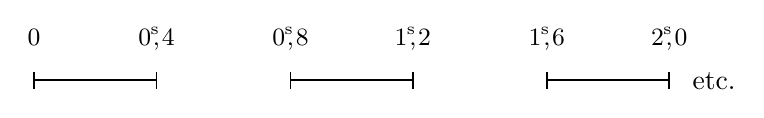
\begin{tikzpicture}[x=.0074cm,y=.0074cm,inner sep=0pt,outer sep=0pt,line width=.65pt]
\node[font=\small,anchor=base] at (0,60) {0};
\node[font=\small,anchor=base] at (210,60) {\GerlingSeconds{0}{4}};
\node[font=\small,anchor=base] at (440,60) {\GerlingSeconds{0}{8}};
\node[font=\small,anchor=base] at (650,60) {\GerlingSeconds{1}{2}};
\node[font=\small,anchor=base] at (880,60) {\GerlingSeconds{1}{6}};
\node[font=\small,anchor=base] at (1090,60) {\GerlingSeconds{2}{0}};
\draw (0,0)--(210,0) (0,-15)--(0,15) (210,-15)--(210,15);
\draw (440,0)--(650,0) (440,-15)--(440,15) (650,-15)--(650,15);
\draw (880,0)--(1090,0) (880,-15)--(880,15) (1090,-15)--(1090,15);
\node[anchor=base west] at (1130,-15) {etc.};
\end{tikzpicture}\par}
\par\noindent\hspace*{\parindent}Doch bemerke ich dabei, dass die Bedeckungen immer recht vollständig sein und eher etwas länger dauern müssen als die Öffnungen; ich meine so:
\par\smallskip
{\centering
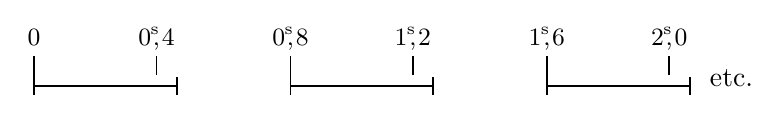
\begin{tikzpicture}[x=.0074cm,y=.0074cm,inner sep=0pt,outer sep=0pt,line width=.65pt]
\node[font=\small,anchor=base] at (0,70) {0};
\node[font=\small,anchor=base] at (210,70) {\GerlingSeconds{0}{4}};
\node[font=\small,anchor=base] at (440,70) {\GerlingSeconds{0}{8}};
\node[font=\small,anchor=base] at (650,70) {\GerlingSeconds{1}{2}};
\node[font=\small,anchor=base] at (880,70) {\GerlingSeconds{1}{6}};
\node[font=\small,anchor=base] at (1090,70) {\GerlingSeconds{2}{0}};
\draw (0,0)--(245,0) (0,-15)--(0,15) (245,-15)--(245,15);
\draw (440,0)--(685,0) (440,-15)--(440,15) (685,-15)--(685,15);
\draw (880,0)--(1125,0) (880,-15)--(880,15) (1125,-15)--(1125,15);
\draw (0,15)--(0,52) (210,20)--(210,52) (440,15)--(440,52) (650,20)--(650,52) (880,15)--(880,52) (1090,20)--(1090,52);
\node[anchor=base west] at (1160,-1) {etc.};
\end{tikzpicture}\par}
\par\noindent\hspace*{\parindent}Andere Zeichen gebe ich mit Zahlen, also zum Beispiel die Zahl 3, nach folgendem Schema:
\par\noindent\hspace*{\parindent}\textls[120]{Ich} Attentionszeichen von unbestimmter Anzahl, bis\\
\hspace*{\parindent}\textls[120]{Sie} dieselben erwiedern und zwar so lange, bis\\
\hspace*{\parindent}\textls[120]{Ich} aufhöre, worauf Sie auch aufhören und \textls[120]{Acht} geben.
Inzwischen mag etwa \(\frac{1}{4}\) Minute gewartet werden.
Dann gebe ich das Zeichen selbst und zwar so:
\par\smallskip
{\centering
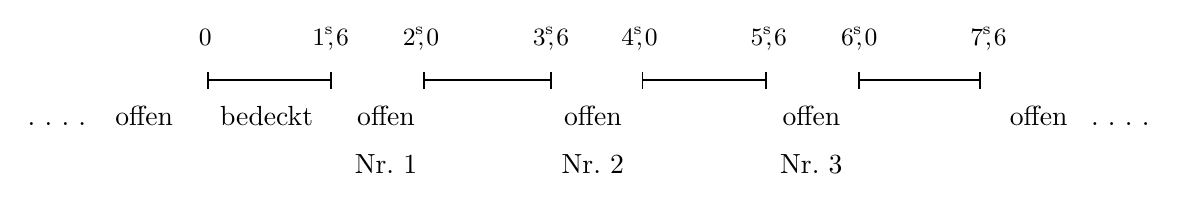
\begin{tikzpicture}[x=.0074cm,y=.0074cm,inner sep=0pt,outer sep=0pt,line width=.65pt]
\node[font=\small,anchor=base] at (360,60) {0};
\node[font=\small,anchor=base] at (575,60) {\GerlingSeconds{1}{6}};
\node[font=\small,anchor=base] at (730,60) {\GerlingSeconds{2}{0}};
\node[font=\small,anchor=base] at (953,60) {\GerlingSeconds{3}{6}};
\node[font=\small,anchor=base] at (1105,60) {\GerlingSeconds{4}{0}};
\node[font=\small,anchor=base] at (1327,60) {\GerlingSeconds{5}{6}};
\node[font=\small,anchor=base] at (1482,60) {\GerlingSeconds{6}{0}};
\node[font=\small,anchor=base] at (1704,60) {\GerlingSeconds{7}{6}};
\draw (365,0)--(575,0) (365,-15)--(365,15) (575,-15)--(575,15);
\draw (735,0)--(953,0) (735,-15)--(735,15) (953,-15)--(953,15);
\draw (1110,0)--(1322,0) (1110,-15)--(1110,15) (1322,-15)--(1322,15);
\draw (1482,0)--(1690,0) (1482,-15)--(1482,15) (1690,-15)--(1690,15);
\node[anchor=base west] at (55,-78) {\mbox{.\ .\ .\ .}};
\node[anchor=base] at (255,-78) {offen};
\node[anchor=base] at (465,-78) {bedeckt};
\node[anchor=base] at (670,-78) {offen};
\node[anchor=base] at (1025,-78) {offen};
\node[anchor=base] at (1400,-78) {offen};
\node[anchor=base] at (1790,-78) {offen};
\node[anchor=base west] at (1880,-78) {\mbox{.\ .\ .\ .}};
\node[anchor=base] at (670,-160) {Nr.~1};
\node[anchor=base] at (1025,-160) {Nr.~2};
\node[anchor=base] at (1400,-160) {Nr.~3};
\end{tikzpicture}\par}
\par\noindent\hspace*{\parindent}Die Zahl also \(=n\) gesetzt, wechseln
\par\smallskip
{\centering
\begin{tabular}{@{}r@{\quad}c@{\quad}l@{}}
 & \(n+1\) & mal bedeckt, 4 Schläge lang,\\
mit & \(n\) & mal offen, 1 Schlag lang (quasi \(n\) Blitze);
\end{tabular}\par}
\smallskip\noindent vorher und nachher, wie bestimmt, infinite quasi offen.
\par\noindent\hspace*{\parindent}Nachher wiederholen Sie dasselbe Manöver umgekehrt; nur, insofern nicht \textls[120]{lange} Unterbrechung stattgefunden hat, ohne meine Erwiederung Ihres Attentionszeichens abzuwarten, sondern nachdem Sie dasselbe etwa 10 bis 20-mal gemacht haben, pausiren Sie (offen) \(\frac{1}{4}\) Minute lang und geben das Zeichen.
\par\noindent\hspace*{\parindent}Doppelte Zeichen, z.~B. \(3\,.\,3\), werden durch doppeltes Attentionszeichen angekündigt (\GerlingSeconds{0}{8} offen und \GerlingSeconds{0}{8} zu), und nachdem die erste Zahl gegeben ist, etwa 5 bis \(10^{\mathrm{s}}\) lang offen gelassen und dann die zweite Zahl gegeben, also
\par\smallskip\noindent\hspace*{.035\linewidth}{\scriptsize IX.}\hfill{\normalsize49}\hspace*{.14\linewidth}\par
\clearpage
\noindent\makebox[0pt][l]{\fontsize{13}{16}\selectfont 386}\hfill{\small\textbf{BRIEFWECHSEL MIT GERLING.}}\hfill\null\par\medskip
{\centering
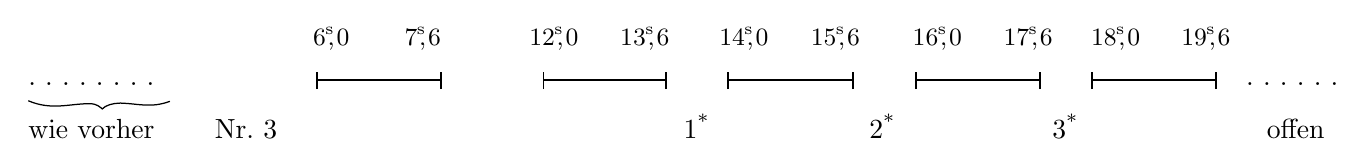
\begin{tikzpicture}[x=.0074cm,y=.0074cm,inner sep=0pt,outer sep=0pt,line width=.65pt]
\node[font=\small,anchor=base] at (540,60) {\GerlingSeconds{6}{0}};
\node[font=\small,anchor=base] at (697,60) {\GerlingSeconds{7}{6}};
\node[font=\small,anchor=base] at (922,60) {\GerlingSeconds{12}{0}};
\node[font=\small,anchor=base] at (1078,60) {\GerlingSeconds{13}{6}};
\node[font=\small,anchor=base] at (1248,60) {\GerlingSeconds{14}{0}};
\node[font=\small,anchor=base] at (1405,60) {\GerlingSeconds{15}{6}};
\node[font=\small,anchor=base] at (1580,60) {\GerlingSeconds{16}{0}};
\node[font=\small,anchor=base] at (1736,60) {\GerlingSeconds{17}{6}};
\node[font=\small,anchor=base] at (1886,60) {\GerlingSeconds{18}{0}};
\node[font=\small,anchor=base] at (2041,60) {\GerlingSeconds{19}{6}};
\draw (516,0)--(728,0) (516,-15)--(516,15) (728,-15)--(728,15);
\draw (904,0)--(1115,0) (904,-15)--(904,15) (1115,-15)--(1115,15);
\draw (1221,0)--(1435,0) (1221,-15)--(1221,15) (1435,-15)--(1435,15);
\draw (1544,0)--(1756,0) (1544,-15)--(1544,15) (1756,-15)--(1756,15);
\draw (1846,0)--(2058,0) (1846,-15)--(1846,15) (2058,-15)--(2058,15);
\node[anchor=base west] at (20,-8) {\mbox{.\ .\ .\ .\ .\ .\ .\ .}};
\draw[line width=.45pt] (20,-35) .. controls (60,-52) and (90,-40) .. (125,-40) .. controls (139,-40) and (144,-47) .. (147,-49) .. controls (152,-43) and (165,-39) .. (178,-39) .. controls (210,-40) and (230,-48) .. (263,-36);
\node[anchor=base west] at (20,-100) {wie vorher};
\node[anchor=base west] at (340,-100) {Nr.~3};
\node[anchor=base] at (1167,-100) {1\textsuperscript{*}};
\node[anchor=base] at (1486,-100) {2\textsuperscript{*}};
\node[anchor=base] at (1800,-100) {3\textsuperscript{*}};
\node[anchor=base west] at (2110,-8) {\mbox{.\ .\ .\ .\ .\ .}};
\node[anchor=base] at (2195,-100) {offen};
\end{tikzpicture}\par}
\par\noindent\hspace*{\parindent}Den Tag des Anfangs überlasse ich, wie schon gesagt, Ihnen.
Nur muss ich so früh davon benachrichtigt werden, dass ich nach Empfang Ihres Briefes noch wenigstens 4 bis 5 Tage habe, um meine Gehülfen in Hannover zu beordern (denn jetzt ruhen die Geschäfte ganz), damit diese auch zur rechten Zeit am Platze sind.
\par\noindent\hspace*{\parindent}Noch Einen Umstand muss ich erwähnen.
Die Gehülfen auf dem Hohehagen und Meisner und eventualiter, sobald ich auf dem Hohehagen bin, der auf dem Brocken, haben nach 2 Richtungen Licht zu schicken, also alternative.
\par\noindent\hspace*{\parindent}Sie werden das nun pro aequo vertheilen, einmal einem 1 Stunde oder 2, dann dem andern.
Allein es wird gut sein, dass solche jedesmal, wo sie die Absicht haben zu wechseln, dies etwa 5 Minuten vorher durch ein \(\frac{1}{2}\) Minute dauerndes Attentionszeichen ankündigen, damit [d]er [Beobachter] durch das plötzliche Abbrechen nicht in einer Beobachtungsreihe im Stiche gelassen zu werden risquire, sondern sie erst gehörig schliessen könne.
Während ich auf dem Hohehagen bin, könnte Ihr Gehülfe mir auch wohl vom Meisner aus zuweilen Licht geben.
Inzwischen werde ich vermuthlich auch den Stein selbst pointiren können, sobald ich einmal weiss, wo er steht, \textls[120]{wenn} er, warum ich bitte, \textls[120]{schwarz} gefärbt ist (mit Theer).
Doch muss dann der Gehülfe nicht unmittelbar am Stein stehen.
Geben Sie ihm also auf, dann, besonders \textls[120]{immer} wenn die Sonne nicht scheint, und, wenn sie scheint, jedesmal, nachdem der Heliotrop eben eingestellt ist, sich auf ein Dutzend Schritte von der Richtung zum Hohehagen seitwärts zu halten.
Vielleicht geben Sie ihm auch auf, schon früher einmal Licht nach Göttingen zu schicken.
Es soll vom 18.~d.~M. an täglich zwischen 2 und \(2\frac{1}{2}\) Uhr aufgepasst und Empfang von Licht durch Erwiederung angezeigt werden.
Ich fürchte aber, dass Ihr Gehülfe Mühe haben wird, die Richtung heraus zu finden.
Wüsste ich die Stelle, so würde ich das Licht durch eigenes herlocken.
Bis jetzt kann ich aber auf dem Gipfel mit dem Teleskop nichts Steinähnliches sehen.
Die höchste Stelle des Meisner ist hier als ein (im verticalen Sinn) schmaler Saum, und als kahle Blösse über Holz her sichtbar.
\par\clearpage
\noindent\null\hfill{\small\textbf{ZUR HANNOVERSCHEN TRIANGULATION.}}\hfill\makebox[0pt][r]{\fontsize{13}{16}\selectfont 387}\par\medskip
\par\noindent\hspace*{\parindent}In dem Fall Nr.~4 würden Sie Ihre Ankunft auf dem Inselsberg dem Gehülfen auf dem Hohehagen durch einmalige Lichtsendung kund thun.
Er liegt \(98^{0}\,28^{\prime}\) links von der Seeberger Sternwarte.
\par\noindent\hspace*{\parindent}Ich gebe Ihnen anheim, ob Sie auch, wenn ich auf dem Hils bin, mir noch einmal Licht vom Meisner dahin schicken lassen wollen.
Es würde immer zur vollständigen Verbindung beitragen.
Herausfordern wollte ich das selber schon, da ich bis dahin den Platz scharf genug kennen werde.
\par\noindent\hspace*{\parindent}Wenn es möglich ist, soll das Heliotroplicht, von dem Platz, wo ich eben selbst messe, im genauen Alignement mit dem Dreieckspunkt sein; geht dies z.~B. auf dem Brocken nicht an, so wird natürlich die Abweichung genau gemessen.
\par\noindent\hspace*{\parindent}Am Hercules habe ich vom Hohehagen aus den Kopf pointirt; vom Brocken aus ist der Hercules nur 4-mal geschnitten und auf die ganze Station oder richtiger auf die ganze pyramidalische Spitze des Oktogons pointirt. --- Vom Hohehagen aus ist zwar der Knill unsichtbar; ich vermuthe aber, dass Amöneburg sichtbar ist, vielleicht auch \mbox{Hohelohr.\quad.\ .\ .\ .\ .\ .}
\par
\endgroup
